\documentclass[journal,10pt]{IEEEtran}

\usepackage{amsmath,amssymb}
\usepackage{dsfont}
\usepackage{graphicx}
\usepackage{booktabs}
\usepackage{cite}
\usepackage{url}
\usepackage{balance}
\usepackage{newtxtext,newtxmath}

\title{Predictability-Aware Sparse Subcarrier Hopping With Bayesian
Reliability-Weighted Decoding Against Delayed Reactive Jamming}

\author{Anonymous Authors}

\begin{document}
\maketitle

\begin{abstract}
Sparse subcarrier hopping can evade a delayed reactive jammer, but hard
recent-set exclusion can also make the next eligible set more predictable. This
paper studies that tradeoff on a common OFDM grid through memory-constrained
sparse hopping (MCSH), predictability-aware soft hopping (PASH), and Bayesian
reliability weighting (BRW). MCSH selects the least recently used active bins
and, if $(L_h+1)S\leq N$, eliminates steady-state collisions from any follower
whose delay does not exceed $L_h$. Stress tests reveal the cost of this hard
rule: collision spikes can appear just outside the design memory and a
candidate-aware jammer can exploit the reduced eligible pool. PASH therefore
uses softened recent-use penalties and an optional inclusion-probability cap,
trading perfect one-slot avoidance for lower worst-lag exposure. BRW
marginalizes the unknown QPSK symbol under clean and jammed variance
hypotheses, while an exact mixture-LLR decoder is used as a receiver benchmark.
Across 251 baseline points and 60 adversarial stress points, MCSH reduces
one-slot follower collision from approximately 0.125 to the acquisition-only
level of 0.016. Under candidate-aware and best-lag attacks, however,
MCSH+mixture-LLR has BLER 0.142 and 0.208, whereas capped PASH reduces them to
0.083 and 0.050, respectively. The results identify both a usable
low-complexity design and the conditions under which it should not be claimed
secure.
\end{abstract}

\begin{IEEEkeywords}
Anti-jamming communications, frequency hopping, OFDM, reactive jamming,
reliability-weighted decoding, sparse multicarrier signaling.
\end{IEEEkeywords}

\section{Introduction}
Reactive and spectrum-aware jammers challenge conventional frequency hopping
(FH) because they sense the legitimate waveform and redirect interference
toward its current or recent frequencies. Recent work addresses the problem
using index-modulated FH \cite{shi2021,shi2022enhanced}, data-driven FH-OFDM
\cite{zhou2024}, reinforcement learning (RL) \cite{zhang2024block,qi2024,cheng2025},
and anti-jamming games \cite{zhang2024game}. Parallel work improves coded
OFDM-IM \cite{kaplan2023,chen2023}, reactive-jammer detection
\cite{altun2022reactive,li2024,wesolowski2023detection}, and robust channel
estimation \cite{mendonca2024channel}.

A separate sequence-design literature studies wide-gap and no-hit-zone FH
sequences \cite{shu2024widegap,zheng2025widegap}. Those constructions establish
valuable correlation and spacing guarantees, but a sparse multicarrier symbol
activates a \emph{set} of frequencies simultaneously. Its collision behavior,
conditional pattern entropy, and interaction with coded soft decoding are not
captured by a scalar FH sequence alone. Moreover, anti-jamming comparisons can
conflate different physical bandwidths, power, coding, or jammer knowledge.

This paper starts from a controlled common-grid baseline and develops a joint
transmitter--receiver method rather than claiming a universal FH processing
gain. Its contributions are:
\begin{itemize}
\item A randomized, set-valued MCSH construction is formulated for sparse
OFDM. A simple feasibility condition and follower-collision law show exactly
when an $L_h$-memory pattern removes delayed reactive collisions.
\item PASH is introduced as a soft, capped alternative to hard exclusion. It
directly targets the predictability failure found in lag-spectrum and
candidate-aware jammer tests.
\item BRW replaces binary erasure with a posterior effective-variance metric.
It is compared with hard erasure, unweighted decoding, oracle erasure, and an
exact clean/jammed mixture-LLR benchmark.
\item The methods are ablated under blind partial-band, sweep, fixed-delay,
random-delay, best-lag, and candidate-aware jammers. Additional experiments
vary actual delay, spectral load, JSR, Pedestrian A/Vehicular A fading, CSI
error, jammer-variance mismatch, and hopping-pattern synchronization error.
\item Failure conditions are reported explicitly: hard MCSH can lose its
advantage outside the design memory, capped PASH sacrifices known one-slot
optimality, and no hopping rule defeats a zero-delay full-information jammer.
\end{itemize}

The contribution is not a claim of inventing no-hit-zone FH, nor a
cryptographic security claim. It is a set-valued sparse-OFDM construction,
collision/predictability analysis, and posterior-weighted coded receiver
evaluated under a single reproducible physical-grid model.

\begin{figure*}[!t]
\centering
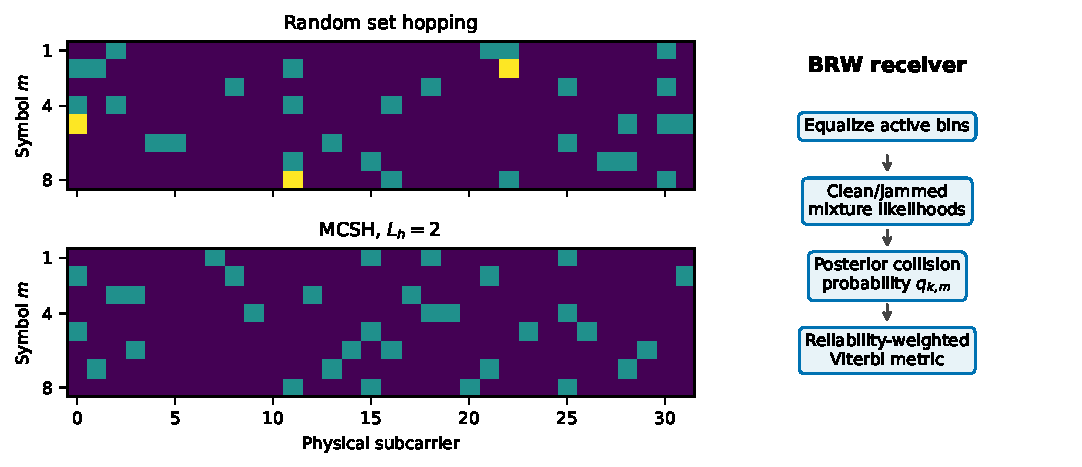
\includegraphics[width=0.98\textwidth]{../figures/paper/fig2_method_concept.pdf}
\caption{MCSH suppresses recent-set reuse while retaining randomized choices.
BRW maps clean/jammed mixture likelihoods to continuous Viterbi reliability
weights. Repeated adjacent bins are highlighted in the random example.}
\label{fig:concept}
\end{figure*}

\section{Related Work and Research Gap}
Table~\ref{tab:related} summarizes the closest research directions. RL and
game-based methods optimize decisions in dynamic environments, but require
training, state design, or online interaction. Enhanced index-modulated FH
specifically targets a power-correlated reactive jammer
\cite{shi2022enhanced}. No-hit-zone sequence work provides strong scalar
sequence constructions \cite{zheng2025widegap}, whereas coded OFDM-IM and
FH-OFDM erasure receivers demonstrate the importance of decoder cooperation
\cite{kaplan2023,chen2023,mailaender2013}. The gap addressed here is a
lightweight set-valued construction with an explicit delayed-follower guarantee
and a non-binary reliability interface to the channel decoder.

\begin{table*}[t]
\centering
\caption{Positioning Relative to Representative Approaches}
\label{tab:related}
\scriptsize
\setlength{\tabcolsep}{2.7pt}
\begin{tabular}{p{2.7cm}p{2.3cm}p{3.2cm}p{3.1cm}p{3.2cm}}
\toprule
Approach & Main object & Reactive-jammer treatment & Coded soft reliability & Main distinction/limit \\
\midrule
RL/game FH \cite{qi2024,zhang2024game,cheng2025} &
Policy/action & Learned or strategic response & Usually external &
Adapts broadly; requires training/state interaction \\
Enhanced IM-FH \cite{shi2022enhanced} &
Index modulation & Power-correlation resistance & Not the main focus &
Targets a different reactive-jammer mechanism \\
Wide-gap/NHZ FHS \cite{shu2024widegap,zheng2025widegap} &
Scalar sequence & Correlation and no-hit-zone bounds & No &
Does not model simultaneous sparse active-bin sets \\
Coded OFDM-IM/FH \cite{kaplan2023,chen2023,mailaender2013} &
Code/erasure & Detection and decoding & Hard/oracle erasure common &
No finite-memory set-collision guarantee \\
This work &
Sparse active-bin set & Finite-memory exclusion & Posterior-weighted Viterbi &
Limited by delay mismatch and pattern synchronization \\
\bottomrule
\end{tabular}
\end{table*}

\section{Common-Grid System and Jammer Model}
\subsection{Sparse OFDM Signal Model}
Consider an allocated OFDM grid of $N$ orthogonal physical bins. At symbol
interval $m$, the transmitter activates a set
$\mathcal{A}_m\subseteq\{0,\ldots,N-1\}$ with $|\mathcal{A}_m|=S$. The same
number of unit-energy QPSK symbols, average power, symbol duration, system-band
allocation, and rate-$1/2$ terminated convolutional code are used by all
compared hopping patterns.

For active bin $k\in\mathcal{A}_m$, the ideal-FFT observation is
\begin{equation}
y_{k,m}=H_k x_{k,m}+\mathds{1}\{k\in\mathcal{J}_m\}z_{k,m}+n_{k,m},
\label{eq:signal}
\end{equation}
where $H_k$ is the communication-channel response,
$n_{k,m}\sim\mathcal{CN}(0,N_0)$, and $\mathcal{J}_m$ is the jammed-bin set.
The jammer has fixed total received energy $S\,10^{\mathrm{JSR}/10}$ per
symbol, divided uniformly across $\mathcal{J}_m$. Define
\begin{equation}
c_m=\frac{|\mathcal{A}_m\cap\mathcal{J}_m|}{S}.
\label{eq:collision}
\end{equation}

\subsection{Jammer Classes}
Four classes are evaluated. Blind partial-band jamming (PBJ) independently
occupies a fraction $\rho$ of the grid. A sweep jammer translates a contiguous
block across symbols. A $d$-slot follower uses
\begin{equation}
\mathcal{J}_m=\mathcal{A}_{m-d},
\label{eq:follower}
\end{equation}
after a random acquisition phase of $d$ symbols. A union follower attacks
$\bigcup_{\ell=1}^{L_j}\mathcal{A}_{m-\ell}$. A zero-delay limit,
$\mathcal{J}_m=\mathcal{A}_m$, is included as an intentionally unfavorable
boundary rather than a scenario the proposed method claims to solve.

Independent random set hopping gives
\begin{equation}
\mathbb{E}[c_m]=\frac{S}{N}
\label{eq:random_collision}
\end{equation}
against a single delayed follower. For blind PBJ,
$\mathbb{E}[c_m]=\rho$ for both independent and memory-constrained patterns;
therefore MCSH should not be expected to create a blind-jammer mean-energy
gain.

\section{Sparse Hopping With Predictability Control}
\subsection{Memory-Constrained Construction}
For candidate physical bin $k$, define its recent-use count
\begin{equation}
r_{k,m}=\sum_{\ell=1}^{\min(L_h,m)}
\mathds{1}\{k\in\mathcal{A}_{m-\ell}\}.
\label{eq:recent}
\end{equation}
MCSH selects the $S$ bins having the smallest $r_{k,m}$, with pseudorandom
tie-breaking generated from a shared seed. Thus, it first uses bins outside
the recent union. If too few such bins exist, it reuses the least recently
occupied bins. The implementation requires no online RL training or jammer
feedback.

\subsection{Collision Guarantee}
\textbf{Proposition 1:} If $(L_h+1)S\leq N$, MCSH produces
\begin{equation}
\mathcal{A}_m\cap
\left(\bigcup_{\ell=1}^{L_h}\mathcal{A}_{m-\ell}\right)=\varnothing
\label{eq:nhz}
\end{equation}
for all valid $m$.

\emph{Proof:} Assume the previous at most $L_h$ sets satisfy the construction.
Their union contains at most $L_hS$ bins, leaving at least
$N-L_hS\geq S$ candidates with $r_{k,m}=0$. MCSH selects $S$ of these
zero-count bins, proving \eqref{eq:nhz}. The initial step is immediate, so the
property follows by induction. \hfill$\square$

\textbf{Corollary 1:} For a $d$-slot follower with $d\leq L_h$, post-acquisition
collision is zero. If the first $d$ jammer sets are independently random, the
frame-average expectation for an $M$-symbol frame is
\begin{equation}
\mathbb{E}[\bar c_{\mathrm{MCSH}}]
=\frac{d}{M}\frac{S}{N},
\quad d\leq L_h,
\label{eq:frame_collision}
\end{equation}
versus $S/N$ for independent random hopping. The same zero steady-state result
holds for a union follower with $L_j\leq L_h$.

The guarantee has two important limits. First, it is infeasible when
$(L_h+1)S>N$. Second, an actual delay beyond $L_h$ is unconstrained and can
occasionally collide more than independent hopping. The delay and load
experiments in Section~\ref{sec:results} test both limits.

\subsection{Predictability-Aware Soft Hopping}
Hard exclusion is optimal against a known $d\leq L_h$ follower, but it exposes
a smaller next-symbol candidate pool. To reduce this predictability, PASH draws
the active set without replacement using softened recent-use weights
\begin{equation}
w_{k,m}=p_{\mathrm{floor}}+
\exp\left(-\alpha\sum_{\ell=1}^{H}
\mathds{1}\{k\in\mathcal{A}_{m-\ell}\}\right),
\label{eq:pash_weight}
\end{equation}
where $H$ is the soft memory, $\alpha$ controls recent-use repulsion, and
$p_{\mathrm{floor}}>0$ prevents deterministic exclusion. The capped variant
further limits the approximate conditional inclusion probability,
\begin{equation}
p_{k,m}=\min\{p_{\max},\eta_m w_{k,m}\},\quad
\sum_{k=1}^{N}p_{k,m}=S,
\label{eq:pash_cap}
\end{equation}
with $\eta_m$ found by bisection. The final set is sampled according to these
weights. Thus, PASH-cap deliberately gives up zero short-delay collision in
exchange for lower worst-lag and candidate-aware exposure.

\subsection{Randomness and Complexity}
When the recent sets are disjoint, the conditional number of next-set choices
is $\binom{N-L_hS}{S}$, giving
\begin{equation}
\mathcal{H}_m=\log_2\binom{N-L_hS}{S}.
\label{eq:entropy}
\end{equation}
For $N=512$, $S=64$, and $L_h=2$, this is approximately 245 bits per symbol.
This is an unpredictability measure under pseudorandom tie-breaking, not a
cryptographic-security proof. Recent-use counting costs
$\mathcal{O}(L_hS+N)$; selecting the lowest-count bins can be implemented in
$\mathcal{O}(N\log S)$. PASH adds one weight pass, a scalar cap search if
\eqref{eq:pash_cap} is used, and weighted sampling without replacement; no
training phase or jammer feedback is required.

\section{Bayesian Reliability-Weighted Decoding}
\subsection{Posterior Collision Probability}
After equalization, let $\widetilde y_{k,m}=y_{k,m}/\widehat H_k$. BRW uses
\begin{align}
\mathcal{H}_0 &: \widetilde y=x+\widetilde n,\quad
\widetilde n\sim\mathcal{CN}(0,v_0),\\
\mathcal{H}_1 &: \widetilde y=x+\widetilde n+\widetilde z,\quad
\widetilde n+\widetilde z\sim\mathcal{CN}(0,v_1),
\end{align}
where $v_1>v_0$. Unlike a nearest-symbol residual test, the unknown QPSK symbol
is marginalized:
\begin{equation}
p_i(\widetilde y)=\frac{1}{4\pi v_i}
\sum_{x\in\mathcal{X}_{\mathrm{QPSK}}}
\exp\left(-\frac{|\widetilde y-x|^2}{v_i}\right).
\label{eq:likelihood}
\end{equation}
With prior collision probability $\pi$, the posterior is
\begin{equation}
q=\Pr(\mathcal{H}_1|\widetilde y)
=\frac{\pi p_1(\widetilde y)}
{\pi p_1(\widetilde y)+(1-\pi)p_0(\widetilde y)}.
\label{eq:posterior}
\end{equation}
Noise variance can be obtained from conventional estimators, while jammer
variance is estimated from sensed interference power. Section~\ref{sec:results}
explicitly varies jammer-variance mismatch.

\subsection{Weighted Viterbi Metric}
BRW forms the effective variance
\begin{equation}
v_{\mathrm{eff}}=(1-q)v_0+qv_1
\label{eq:veff}
\end{equation}
and weights each coded-bit branch metric by $1/v_{\mathrm{eff}}$. For trellis
branch $b$ with expected antipodal coded components $\boldsymbol\mu_b$,
\begin{equation}
\Lambda_b=\sum_j
\frac{(s_j-\mu_{b,j})^2}{v_{\mathrm{eff},j}},
\label{eq:metric}
\end{equation}
where $s_j$ is the QPSK soft component. Hard erasure is recovered by setting
weights to zero when $q>0.5$; oracle erasure uses the true collision mask only
as an upper bound. In the adversarial stress suite we also report an exact
clean/jammed mixture-LLR Viterbi metric that evaluates the two QPSK-mixture
likelihoods for each bit. It is used to avoid overstating PASH or MCSH effects
that are actually caused by receiver suboptimality.

BRW adds eight QPSK distance/exponential terms per active sample and
$\mathcal{O}(SM)$ storage for posterior weights. The constraint-length-7
Viterbi decoder remains dominant with complexity proportional to
$2^{K-1}SM$.

\section{Experimental Methodology}
All experiments are generated by an independent Python implementation and do
not reuse the invalid legacy MATLAB results identified during the project
audit. Table~\ref{tab:parameters} lists the default configuration.

\begin{table}[t]
\centering
\caption{Default Experimental Configuration}
\label{tab:parameters}
\scriptsize
\setlength{\tabcolsep}{3pt}
\begin{tabular}{p{2.6cm}p{5.0cm}}
\toprule
Parameter & Value \\
\midrule
Physical grid / active bins & $N=512$, $S=64$ \\
Symbols per frame & $M=8$ \\
Modulation and code & QPSK; terminated rate-$1/2$ K7 $(171,133)_8$ \\
Default SNR / JSR & $E_s/N_0=12$ dB / JSR=5 dB \\
PBJ / sweep occupancy & $0.25N$ / $0.125N$ \\
Sweep step & 24 bins per symbol \\
MCSH memory & $L_h=2$ unless varied \\
Channels & AWGN, Pedestrian A, Vehicular A \\
Core / robustness frames & 300 / 200 per point \\
Adversarial stress & 30 seeds $\times$ 5000 symbols; 240 frames per coded point \\
Uncertainty reporting & Wilson 95\% BER confidence intervals \\
\bottomrule
\end{tabular}
\end{table}

The core study separates pattern and receiver effects using random+K7,
random+BRW, MCSH+K7, MCSH+hard erasure, MCSH+BRW, and MCSH+oracle erasure.
The 251-point suite contains 63,000 frames and approximately 32.8 million
information bits. It additionally varies follower delay $d=1,\ldots,6$, memory
$L_h\in\{1,2,4,6\}$, JSR from $-5$ to 15 dB, active load, channel profile, CSI
NMSE, jammer-variance error, and erroneous-pattern probability. A pattern
desynchronization event shifts all receiver bin indices for that OFDM symbol,
which models a severe mapping error rather than a mild phase offset.

The adversarial suite adds two tests that are closer to a publishable
stress-test standard. First, continuous long-run hopping sequences over 30
seeds and 5000 OFDM symbols per seed estimate the lag-collision spectrum,
worst-lag collision, candidate-aware collision, and bin-usage coefficient of
variation. Second, 60 coded points report BLER and collision rate for random,
MCSH, PASH, and capped PASH under fixed one-slot, fixed three-slot, random
delay, best-lag, and candidate-aware jammers. Each point compares no weighting,
BRW, and exact mixture-LLR decoding.

Finally, model-validity checks verify structural invariants before interpreting
BER or BLER: random hopping matches the closed-form load $S/N$, MCSH has zero
lag-1 and lag-2 collision for $L_h=2$, worst-lag spikes occur at $L_h+1$, and
PASH-cap reduces the maximum of worst-lag and candidate-aware exposure while
sacrificing zero short-delay collision. All nine checks pass.

\begin{figure*}[!t]
\centering
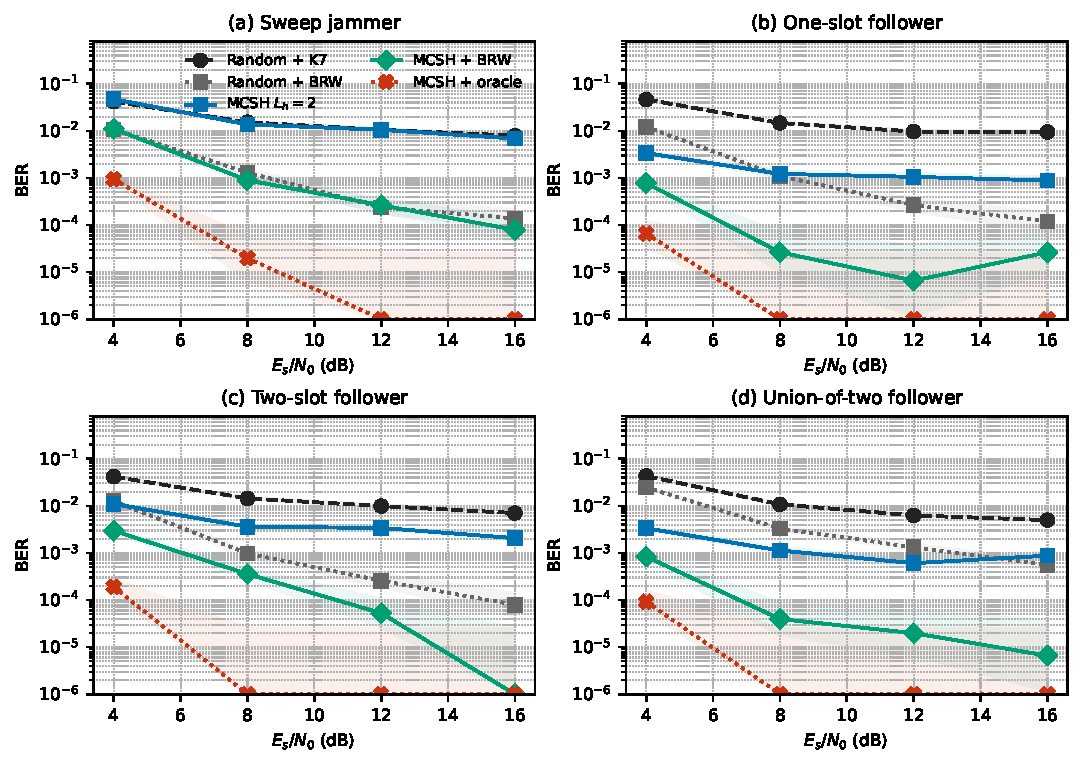
\includegraphics[width=\textwidth]{../figures/paper/fig3_core_method.pdf}
\caption{Core BER results at JSR=5 dB. Curves at the $10^{-6}$ plotting floor
with zero measured errors must be interpreted through their Wilson upper
confidence bounds, not as zero true BER.}
\label{fig:core}
\end{figure*}

\section{Results and Discussion}
\label{sec:results}
\subsection{Separating Pattern and Receiver Gains}
Figure~\ref{fig:core}(a) shows that MCSH alone does not improve sweep-jammer
mean collision or BER, as expected because the sweep is unrelated to recent
active sets. BRW, however, reduces the sweep BER from approximately
$10^{-2}$ to the $10^{-4}$ range at 12 dB. This is a receiver gain, not an
MCSH gain. Blind PBJ gives the same conclusion: the pattern does not lower mean
collision, whereas BRW retains useful soft information that hard erasure can
discard.

For one- and two-slot followers, MCSH changes the collision mechanism.
At $S/N=1/8$, independent hopping collides at approximately 0.125. With
$L_h=2$, measured frame-average collision is approximately 0.016 for $d=1$
and 0.032 for $d=2$, agreeing with \eqref{eq:frame_collision}. The remaining
collisions arise only from the deliberately random acquisition symbols. The
union-of-two follower is similarly reduced from roughly 0.21 to 0.015.

\begin{table*}[t]
\centering
\caption{Representative Results at $E_s/N_0=12$ dB and JSR=5 dB}
\label{tab:keyresults}
\scriptsize
\setlength{\tabcolsep}{5pt}
\begin{tabular}{l l c c c}
\toprule
Jammer / condition & Scheme & Collision rate & BER & Wilson 95\% interval \\
\midrule
Sweep & MCSH+K7 & 0.125 & $1.053\times10^{-2}$ & $[1.003,1.106]\times10^{-2}$ \\
Sweep & MCSH+hard erasure & 0.125 & $4.216\times10^{-4}$ & $[3.302,5.383]\times10^{-4}$ \\
Sweep & MCSH+BRW & 0.125 & $2.635\times10^{-4}$ & $[1.935,3.588]\times10^{-4}$ \\
One-slot follower & random+K7 & 0.124 & $9.677\times10^{-3}$ & $[9.197,10.182]\times10^{-3}$ \\
One-slot follower & MCSH+K7 & 0.016 & $1.054\times10^{-3}$ & $[0.903,1.230]\times10^{-3}$ \\
One-slot follower & MCSH+BRW & 0.016 & $6.588\times10^{-6}$ & $[1.163,37.317]\times10^{-6}$ \\
Union-of-two follower & random+K7 & 0.206 & $6.258\times10^{-3}$ & $[5.874,6.668]\times10^{-3}$ \\
Union-of-two follower & MCSH+BRW & 0.015 & $1.976\times10^{-5}$ & $[0.672,5.811]\times10^{-5}$ \\
\bottomrule
\end{tabular}
\end{table*}

\begin{figure*}[!t]
\centering
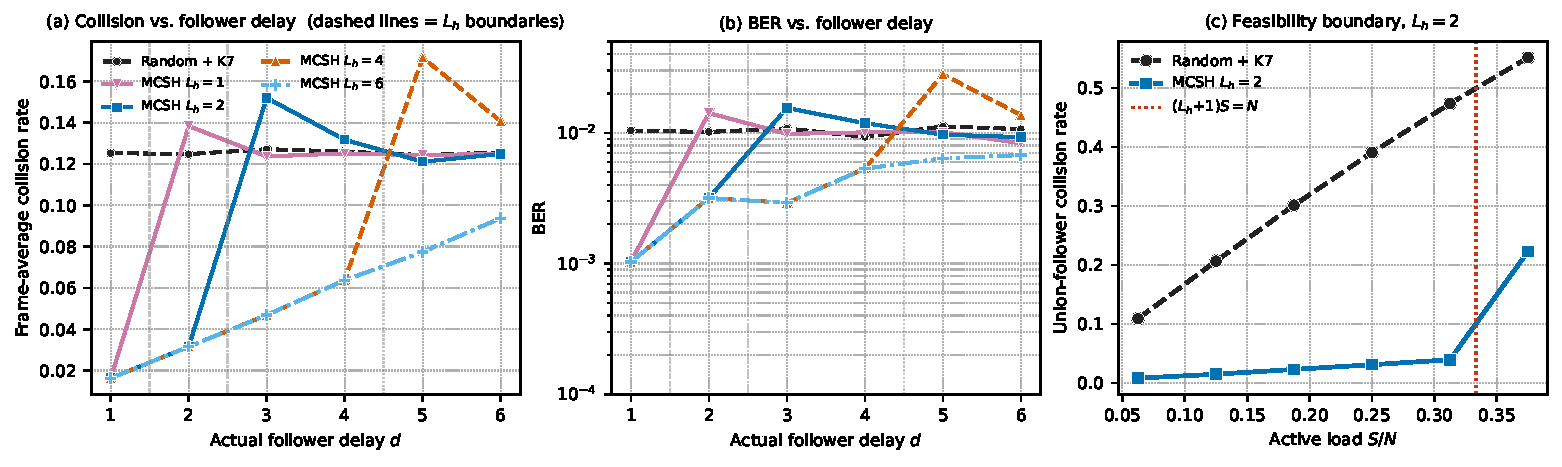
\includegraphics[width=\textwidth]{../figures/paper/fig4_delay_load.pdf}
\caption{Memory and load ablation at $E_s/N_0=12$ dB and JSR=5 dB. A memory
chosen shorter than the actual delay can be worse than random hopping. The
vertical line marks the zero-recent-overlap feasibility boundary for $L_h=2$.}
\label{fig:delay}
\end{figure*}

\subsection{Memory Depth and Feasibility Boundary}
Figure~\ref{fig:delay}(a) verifies the acquisition-only law for every
$d\leq L_h$. It also shows the cost of mismatch. For example, $L_h=2$ has
higher collision than random hopping at $d=3$ because the construction only
controls the two most recent sets. Increasing memory protects a larger delay
range, but reduces the conditional choice count in \eqref{eq:entropy}.

The load sweep in Fig.~\ref{fig:delay}(c) tests $(L_h+1)S\leq N$. MCSH remains
near its acquisition floor through $S=160$ for $N=512$, but collision rises
sharply at $S=192$, beyond the $S/N=1/3$ feasibility boundary. This prevents
the zero-collision property from being overgeneralized to heavily loaded
multicarrier systems.

\begin{figure*}[!t]
\centering
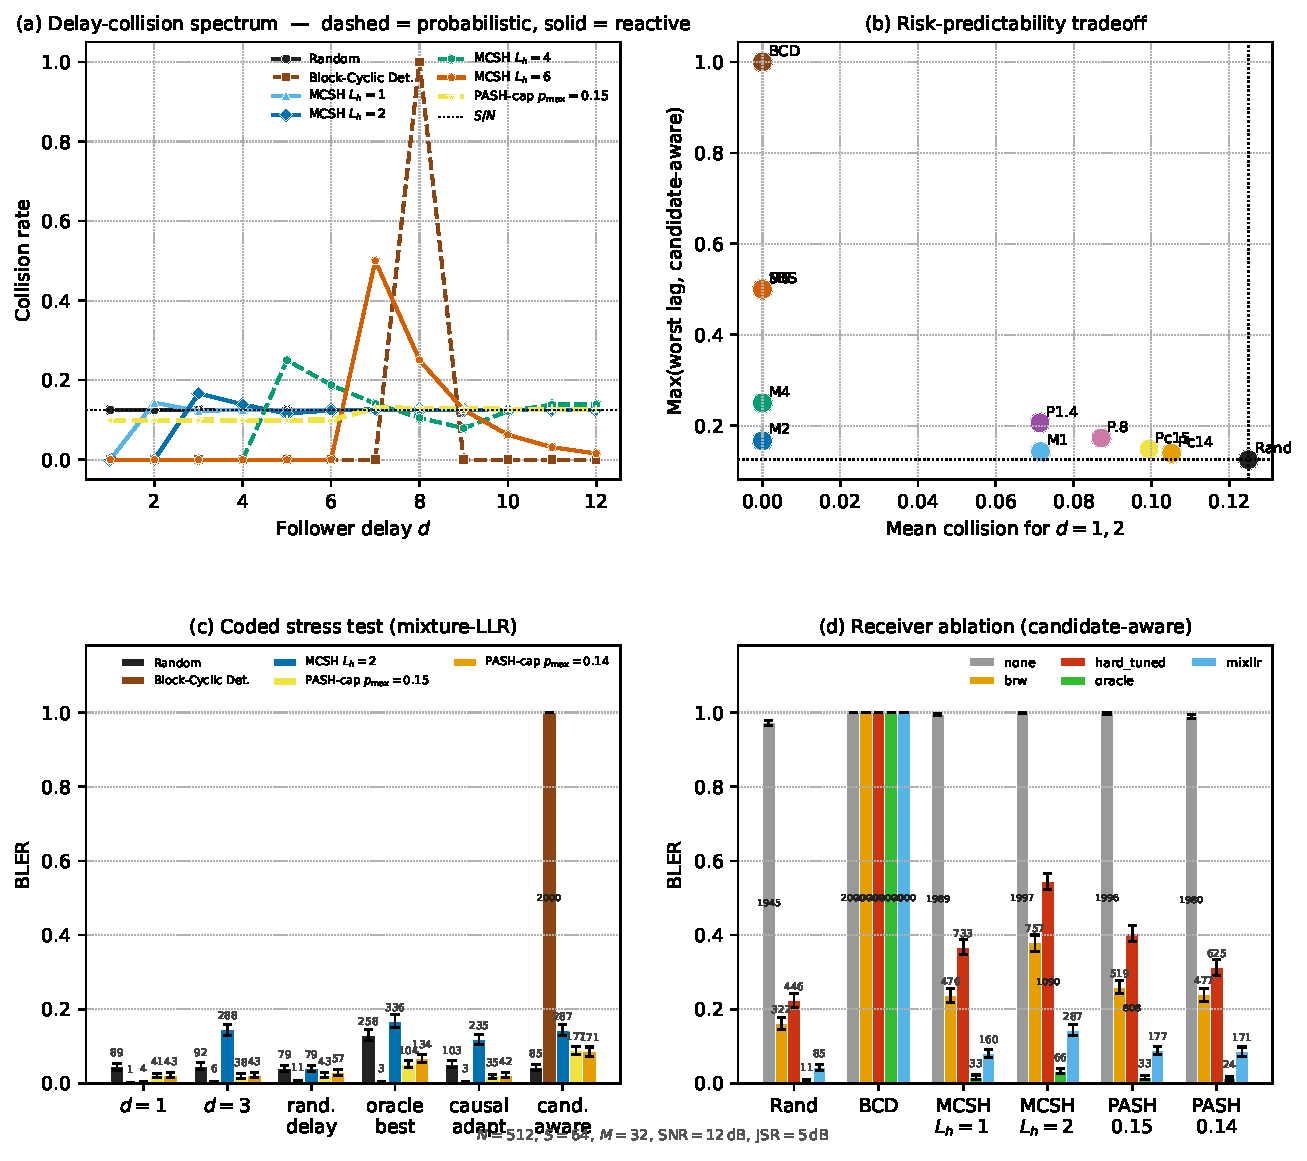
\includegraphics[width=\textwidth]{../figures/paper/fig7_adversarial_pash.pdf}
\caption{Adversarial predictability stress tests. MCSH removes collisions
inside its memory but creates lag spikes just outside it; capped PASH lowers
worst-lag and candidate-aware exposure, then converts the structural gain into
lower BLER under best-lag and candidate-aware jammers.}
\label{fig:pash}
\end{figure*}

\subsection{Adversarial Predictability Stress Tests}
Figure~\ref{fig:pash} addresses the main weakness of hard recent-set exclusion.
Long-run structural tests show that MCSH with $L_h=2$ has zero mean collision
for lags 1--2, but its worst-lag collision rises to 0.167 at lag 3. Increasing
to $L_h=6$ shifts the problem rather than removing it: the worst-lag collision
reaches 0.500 at lag 7 because the eligible pool is extremely concentrated.
These results explain why a delay mismatch can reverse the MCSH gain.

PASH-cap changes the design objective from ``zero collision at selected short
lags'' to ``bounded predictability over many plausible lags.'' Its mean
collision over lags 1--2 is 0.099, so it is worse than MCSH against a perfectly
known one-slot follower. However, its worst-lag collision is 0.130 and its
candidate-aware collision is 0.148, both lower than the MCSH $L_h=2$ values
of 0.167 and 0.167. In coded stress tests with mixture-LLR decoding, this
tradeoff is visible: MCSH has BLER 0.004 for a fixed one-slot follower, but
0.125, 0.208, and 0.142 for fixed three-slot, best-lag, and candidate-aware
jammers. PASH-cap gives 0.029 for the one-slot case, yet reduces those three
stronger attacks to 0.013, 0.050, and 0.083. The result is not that PASH-cap
dominates MCSH; it is that the correct hopping rule depends on the uncertainty
and adversarial knowledge of the jammer delay.

\begin{figure*}[!t]
\centering
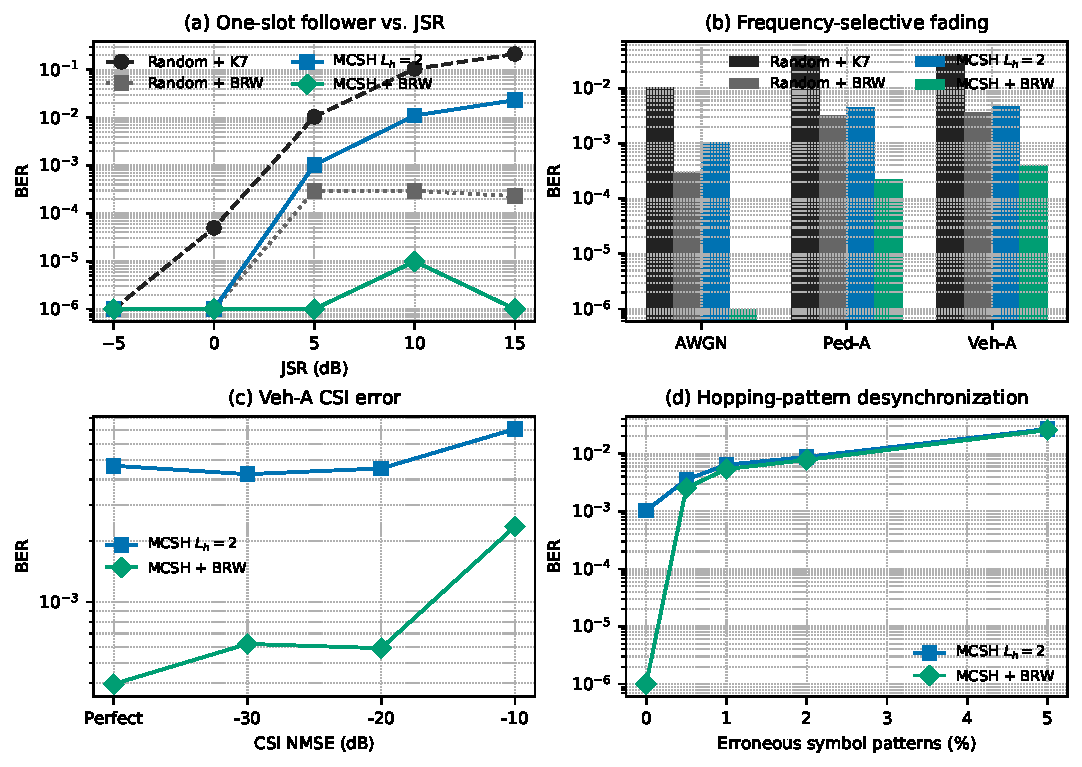
\includegraphics[width=\textwidth]{../figures/paper/fig5_robustness.pdf}
\caption{Robustness experiments for a one-slot follower unless otherwise
noted: JSR, multipath fading, CSI error, and hopping-pattern desynchronization.}
\label{fig:robust}
\end{figure*}

\subsection{JSR, Fading, CSI, and Synchronization}
Figure~\ref{fig:robust}(a) shows different roles for the two modules. MCSH
reduces the number of follower collisions, while BRW prevents the remaining
high-JSR samples from dominating the decoder. In Pedestrian A and Vehicular A
fading, Fig.~\ref{fig:robust}(b) shows that BRW continues to improve both
random and memory-constrained hopping under perfect CSI. With Vehicular A
channel-estimation error, performance degrades gradually through $-10$ dB
NMSE rather than collapsing immediately.

Hopping synchronization is more critical. At a 1\% erroneous-pattern rate,
the MCSH+BRW BER rises into the $10^{-3}$ range, and at 5\% it reaches the
$2.576\times10^{-2}$ level. This experiment uses a full-bin mapping error, so it should
be read as a synchronization-failure bound. A deployable system requires an
authenticated pattern resynchronization mechanism.

\begin{figure*}[!t]
\centering
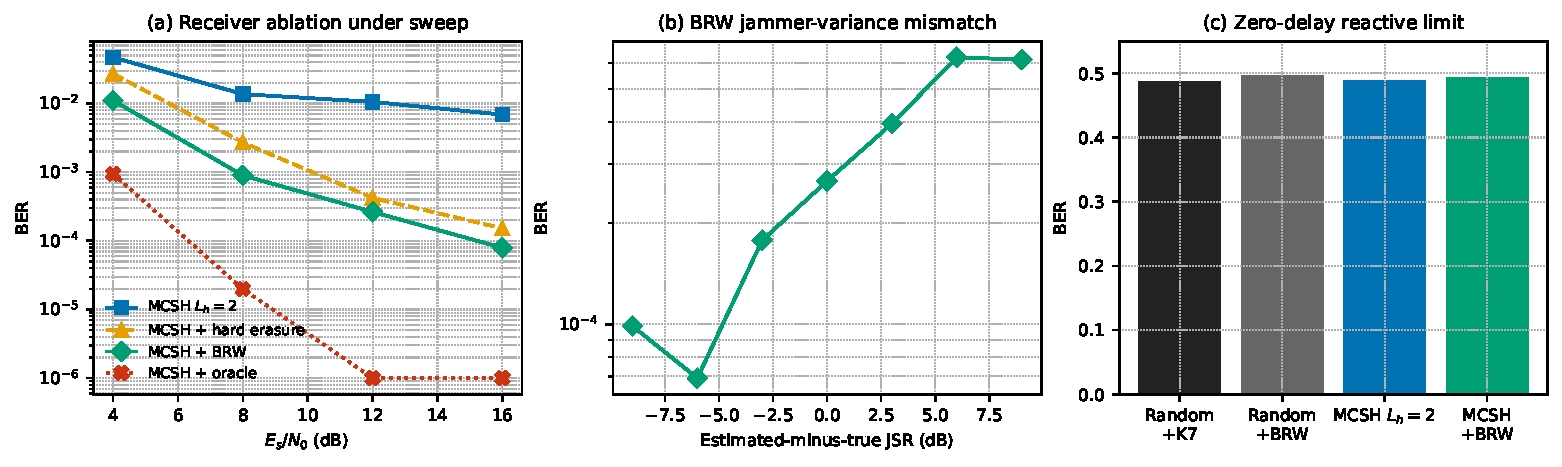
\includegraphics[width=\textwidth]{../figures/paper/fig6_receiver_limits.pdf}
\caption{Receiver ablation, jammer-variance mismatch, and the zero-delay
reactive-jammer limit.}
\label{fig:receiver}
\end{figure*}

\subsection{Receiver Ablation and Failure Boundaries}
Figure~\ref{fig:receiver}(a) compares no weighting, hard erasure, BRW, and
oracle erasure under sweep jamming. BRW consistently improves upon hard
erasure because uncertain samples are downweighted instead of discarded.
The remaining oracle gap identifies posterior modeling and variance estimation
as future receiver opportunities. Figure~\ref{fig:receiver}(b) shows that BRW
remains useful under several decibels of jammer-power estimation error, though
the best point need not occur at zero mismatch because the approximate
two-component model does not represent every sweep sample exactly.

Finally, Fig.~\ref{fig:receiver}(c) gives the necessary negative result:
when the jammer instantaneously occupies $\mathcal{A}_m$, all compared schemes
approach BER 0.5; MCSH+BRW measures 0.494. MCSH is a defense against delayed followers, not a solution
to a zero-latency full-information jammer.

\subsection{Complexity and Practical Interpretation}
MCSH adds a recent-use array and a partial selection per OFDM symbol. BRW adds
constant-order mixture likelihoods per active sample, while the existing
Viterbi decoder remains asymptotically dominant. No-jam experiments show no
systematic BER penalty from the MCSH pattern itself. The main implementation
cost is therefore pattern synchronization and variance estimation rather than
decoder order.

Compared with RL-based approaches, MCSH/PASH-BRW has no training phase and the
MCSH delayed-follower guarantee is explicit. Conversely, RL or game-based
policies can adapt to richer jammer behavior that violates the assumed delay
model. The methods are therefore complementary rather than directly ranked by
a single BER number.

\section{Limitations and Future Work}
The study uses an ideal FFT boundary and frequency-domain jammer model.
Although Pedestrian A/Vehicular A fading, CSI error, and mapping
desynchronization are included, timing offset, CFO-induced intercarrier
interference, pilot overhead, channel coding beyond K7, and hardware nonlinear
effects remain open. The stronger best-lag and candidate-aware tests are still
heuristic adversaries, not a full game-theoretic optimum. Likewise, PASH-cap is
an interpretable capped exponential rule rather than a proven minimax hopping
law. Future work should combine delay-belief estimation, adaptive memory,
authenticated resynchronization, stronger codes, and over-the-air validation.

\section{Conclusion}
Sparse subcarrier hopping against delayed reactive jamming is a joint
collision, predictability, and soft-reliability problem. Under a feasible
spectral load, MCSH removes steady-state collisions from followers within its
design memory; under uncertain or adversarially selected delay, PASH-cap lowers
worst-lag and candidate-aware exposure at the cost of known one-slot
optimality. BRW and mixture-LLR decoding then show how much of that structural
gain survives in a coded receiver. The negative and robustness tests identify
the main boundaries: memory mismatch, excessive active load, zero jammer delay,
and hopping desynchronization. These boundaries make the reported gains more
reproducible and technically defensible.

\vfill
\balance
\bibliographystyle{IEEEtran}
\bibliography{references_ieee}

\end{document}
